\documentclass[a4paper,10pt]{report}
\usepackage[utf8]{inputenc}
\usepackage[T1]{fontenc}
\usepackage{graphicx}
\usepackage{eurosym}
\usepackage[francais]{babel}

\title{Projet Njörd}
\author{AIGREAUL Clément - HENRIO Jordan - PHAM Chitin}

\begin{document}
  \maketitle

  \chapter*{Introduction}
    Nous vivons dans un monde où la technologie a atteint un point permettant de “donner vie” à des objets. Si bien qu’ils
    peuvent prendre des décisions, apprendre et communiquer. Une telle avancée permet des milliers d’applications aussi bien
    pour le divertissement, la domotique, l’industrie, ou encore l’assistance. Parfois l’Homme peut être amené à devoir exécuter
    certaines missions sur des terrains dont on ne possède pas une connaissance exacte (comme par exemple une ville ayant subi
    une catastrophe naturelle). Ainsi un des problèmes majeurs des agents de sécurité est de connaître exactement la situation
    afin de mettre en place une stratégie d’approche. La création d’une équipe de robots permettant l’analyse d’un lieu peut être
    d’une très grande utilité dans ce genre de situation. C'est pourquoi nous avons choisi, dans le cadre de notre projet de fin 
    d'études, de créer une équipe de drones volants qui communiquent ensemble par l'implémentation d'un serveur central qui reçoit
    des informations de la part des drones et qui dessine la topographie de la zone analysée. Ce rapport a pour but de présenter 
    le développement et les choix technologiques de ce projet. Il explique les calculs réalisés pour le choix des composants, 
    les erreurs que nous avons faites et présente les résultats obtenus pendant les phases de tests.
  
  \tableofcontents

  \chapter{Environnement}
    \section{Gestionnaire de version}
      Pour ce projet nous avons choisi de former un groupe de trois personnes. Travailler en équipe a ses avantages, 
      notamment pour le partage de tâches. Mais ceci peut entraîner des problèmes de version entre les travaux de chacun. 
      Pour palier ce problème nous avons choisi d'utiliser le gestionnaire de version Git. Cet outil est vraiment pratique, 
      puisqu'il permet de travailler à distance, de mettre à jour le code de tout le monde, d'avoir un suivi de chaque implémentation, 
      de faire des versions tests (sans toucher à la version fonctionnelle) ou encore de revenir à des versions précédentes du projet.
      Aussi cet outil nous permet de donner une visibilité à notre travail. Ainsi, si une personne compte faire un projet semblable 
      au nôtre il pourra consulter, reprendre, modifier, améliorer... ce que nous avons fait. Notre répertoire Git est accéssible 
      depuis cette adresse\cite{njordgit}.
      
    \section{Communication}
      Dès le début du projet nous avons pensé qu'il serait intéressant de tenir un blog\cite{njordblog} pour communiquer l'avancée
      du projet. Lorsque l'on se lance dans un projet de cette envergure il est toujours utile de trouver des ressources sur Internet.
      Cela peut donner des idées et résoudre des problématiques que l'on rencontre. Afin de pouvoir communiquer avec le plus de monde 
      possible, ce blog est rédigé dans trois langues : anglais, français et japonais. Ce blog présente l'avancée du projet, nos choix
      de développement, quelques notions de physique et les résultats de nos essais afin de guider les lecteur qui veulent créer une 
      application similaire. Nous avons souhaité présenter le processus de construction d'un drone, sous une forme simple, en expliquant
      comment les choses fonctionnent.
      
    \section{Fabrication}
      Pour ce qui est de la fabrication des appareils nous sommes passés par le fablab\cite{faclab} de l'université de Cergy-Pontoise. 
      Cet atelier se trouve à Gennevilliers (92), il propose un grand nombre d'outils mis à disposition gratuitement. La seule 
      contrepartie est de donner de son temps à la vie du laboratoire. Toutefois pour utiliser certaines machines comme les imprimantes
      3D (de qualité), les découpeuses lazer, les fraiseuses, etc... il est nécessaire de suivre une formation. Les gérants étant 
      conscients que nous sommes soumis à des deadlines, nous ont proposé de faire les choses à notre place. En échange on devait 
      simplement faire des formations sur l'utilisation du logiciel Fritzing et sur la fabrication d'un drone.

  \chapter{Premier drone}
    Etant donné notre cursus, nous ne savions pas réellement comment procéder pour monter un drone. Nous avons commencé par nous
    renseigner sur ce qui se fait en matière de drones. Il faut savoir qu'il en existe de plusieurs types, des petits, des grands,
    des appareils avec un vol "agressif" (rapide et agile), d'autres avec un vol optimisé pour la prise de vues, certains avec un 
    vol dit "hybride", etc.
    
    Pour l'application que nous voulons faire nous avons plutôt besoin d'un drone avec un vol hybride. Le but est de dessiner la 
    topographie d'une zone, pour cela nous utilisons un capteur ultrason qui mesure la distance entre le drone et ce qu'il y a en 
    dessous. Nous n'avons donc pas besoin d'un vol assez lent pour faire des prises de vues, mais il ne faut pas que le drone soit 
    trop rapide afin de prendre le plus d'informations possible. De plus, pour des questions pratiques, il faut que le
    drone ait assez d'autonomie pour ne pas demander que sa batterie soit rechargée pendant une session d'analyse.
    
    Parmi les drones déjà existants, le drone \textit{Crazyflie} de chez \textit{Bitcraze}\cite{bitcraze} nous a intéressés par sa
    petite taille (voir Figure \ref{crazyflie}), par le fait qu'il soit libre et qu'on puisse facilement acheter tous les composants 
    séparément. Nous avons donc décidé de baser notre modèle sur ce petit drone. Plus concrètement, le nôtre a une taille similaire
    au Crazyflie et dispose de la même batterie, des mêmes moteurs et des mêmes pales mais le reste des composants sont différents.
    Nous ne voulions pas passer directement par un Crazyflie, car un de nos objectifs est de construire le robot d'A à Z. De plus ce
    modèle n'est pas tout à fait adapter à ce que nous voulons faire, car il est trop léger et est alors trop véloce. 
    Donc dans tous les cas nous aurions été obligés de le modifier.
    
    \begin{figure}[htbp]%Photo du crazyflie
      \centering
      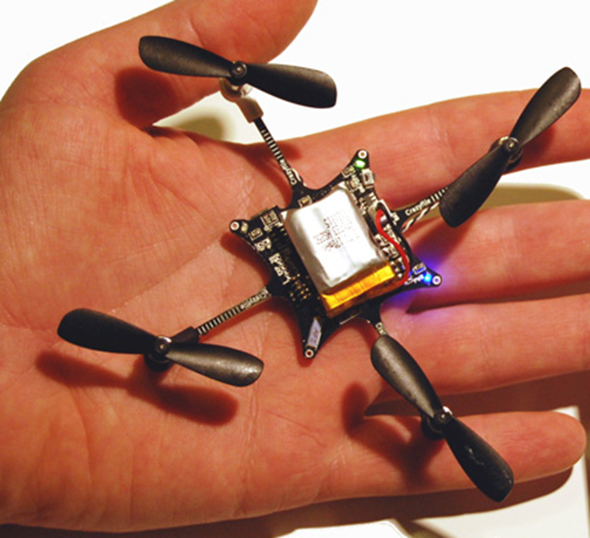
\includegraphics[scale = 0.25]{img/crazyflie.png}
      \caption{Crazyflie}
      \label{crazyflie}
    \end{figure}
    
    \section{Composants}
      L'objectif de cette section est de présenter les différents composants que nous avons utilisés pour construire ce premier drone.
      
      \subsection{Microcontrôlleur}
	Au début de notre année scolaire, nous avons eu un séminaire pour nous apprendre le langage \textit{Arduino}. Nous avons pu 
	découvrir un langage vraiment simple à prendre en main lorsque l'on a déjà quelques bases en programmation avec des langages 
	comme le \textit{C}. Nous nous sommes donc tourné vers les technologies proposés par \textit{Arduino} pour le choix du 
	microcontrôleur. Finalement, nous avons opté pour une \textit{Arduino Pro Mini}. Le principal intérêt de cette carte se trouve
	dans sa petite taille et sa légèreté, 18 sur 33 millimètres pour 2 grammes. De plus elle propose un nombre suffisant de broches 
	pour notre montage.
	
	\begin{figure}[htbp]%Photo de l'Arduino
	  \centering
	  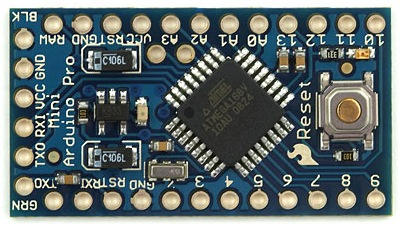
\includegraphics[scale = 0.25]{img/arduinopromini.jpg}
	  \caption{Arduino Pro Mini}
	  \label{arduinopromini}
	\end{figure}	
	
      \subsection{Equilibrage et localisation}
	Il est important de disposer d'une technologie pour assister le drone à se stabiliser. Pour cela, ce dernier doit connaître
	"en permanence" son angle d'inclinaison. Nous avons donc besoin d'un gyroscope. Le large catalogue de modules \textit{Arduino}
	propose une pièce qui fournit un gyroscope et un accéléromètre, le \textit{MPU-6050}. Ce module a une taille et un poids 
	similaires à ceux du microcontrôleur, 25.5 sur 15.2 millimètres pour 1.5 grammes.
	
	Pendant un certain moment nous nous sommes demandé comment nous pourrions connaître la position de notre drone dans l'espace. 
	Naturellement nous avons pensé au GPS, mais la précision de ces technologies (pour rester dans un budget abordable) n'est clairement 
	pas assez précise. Bien entendu, dans le cadre où le drone devrait faire son analyse en extérieur sur une zone assez grande, les 
	GPS sont intéressants. Mais notre drone devra simplement analyser une salle de classe, alors une précision "au mètre près" est 
	beaucoup trop large. Nous aurions plutôt besoin d'une précision de l’ordre du décimètre.  Une autre solution a été évoquée, créer 
	notre propre système de localisation, en créant une triangulation à l’aide d’un réseau d’antennes. Toutefois, pour des raisons de 
	coûts et de poids,  cette solution ne nous semble pas viable sur notre drone. Finalement une connaissance, nous a conseillé de 
	travailler avec un accéléromètre. Un accéléromètre est un module permettant de mesurer l'accélération linéaire d’un système. 
	En connaissant l'accélération de notre drone, il sera alors possible de déterminer sa vitesse et donc, ses déplacements dans 
	l’espace. Nous avons donc choisi de nous tourner vers cette solution.
	
	\begin{figure}[htbp]%Photo de l'accéléromètre
	  \centering
	  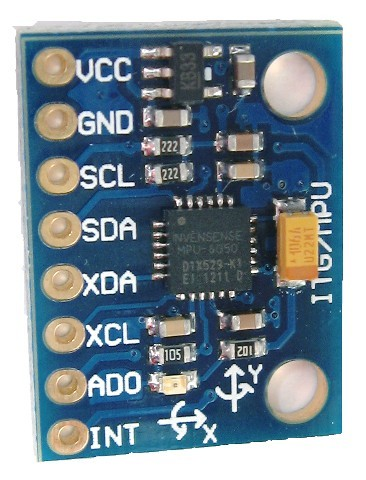
\includegraphics[scale = 0.2]{img/mpu-6050.jpg}
	  \caption{MPU-6050}
	  \label{mpu6050}
	\end{figure}	
      
      \subsection{Communication avec le serveur}
	Afin que le drone puisse communiquer avec le serveur nous avons dans un premier temps pensé à utiliser des modules \textit{XBee}, 
	qui utilisent le protocole de communication sans fil, défini par le standard \textit{IEEE 802.15.4}. Les modules \textit{XBee} 
	étant relativement chers (23 \euro), nous nous sommes penchés vers une autre technologie. Nous avons finalement opté pour un module
	de transmission 2.4GHz. Comme pour les autres composants que nous avons choisis, il est bon marché (0.8 \euro) et d'une taille de 15 
	sur 29 millimètres pour 2 grammes.
	
	\begin{figure}[htbp]%Photo du transmetteur
	  \centering
	  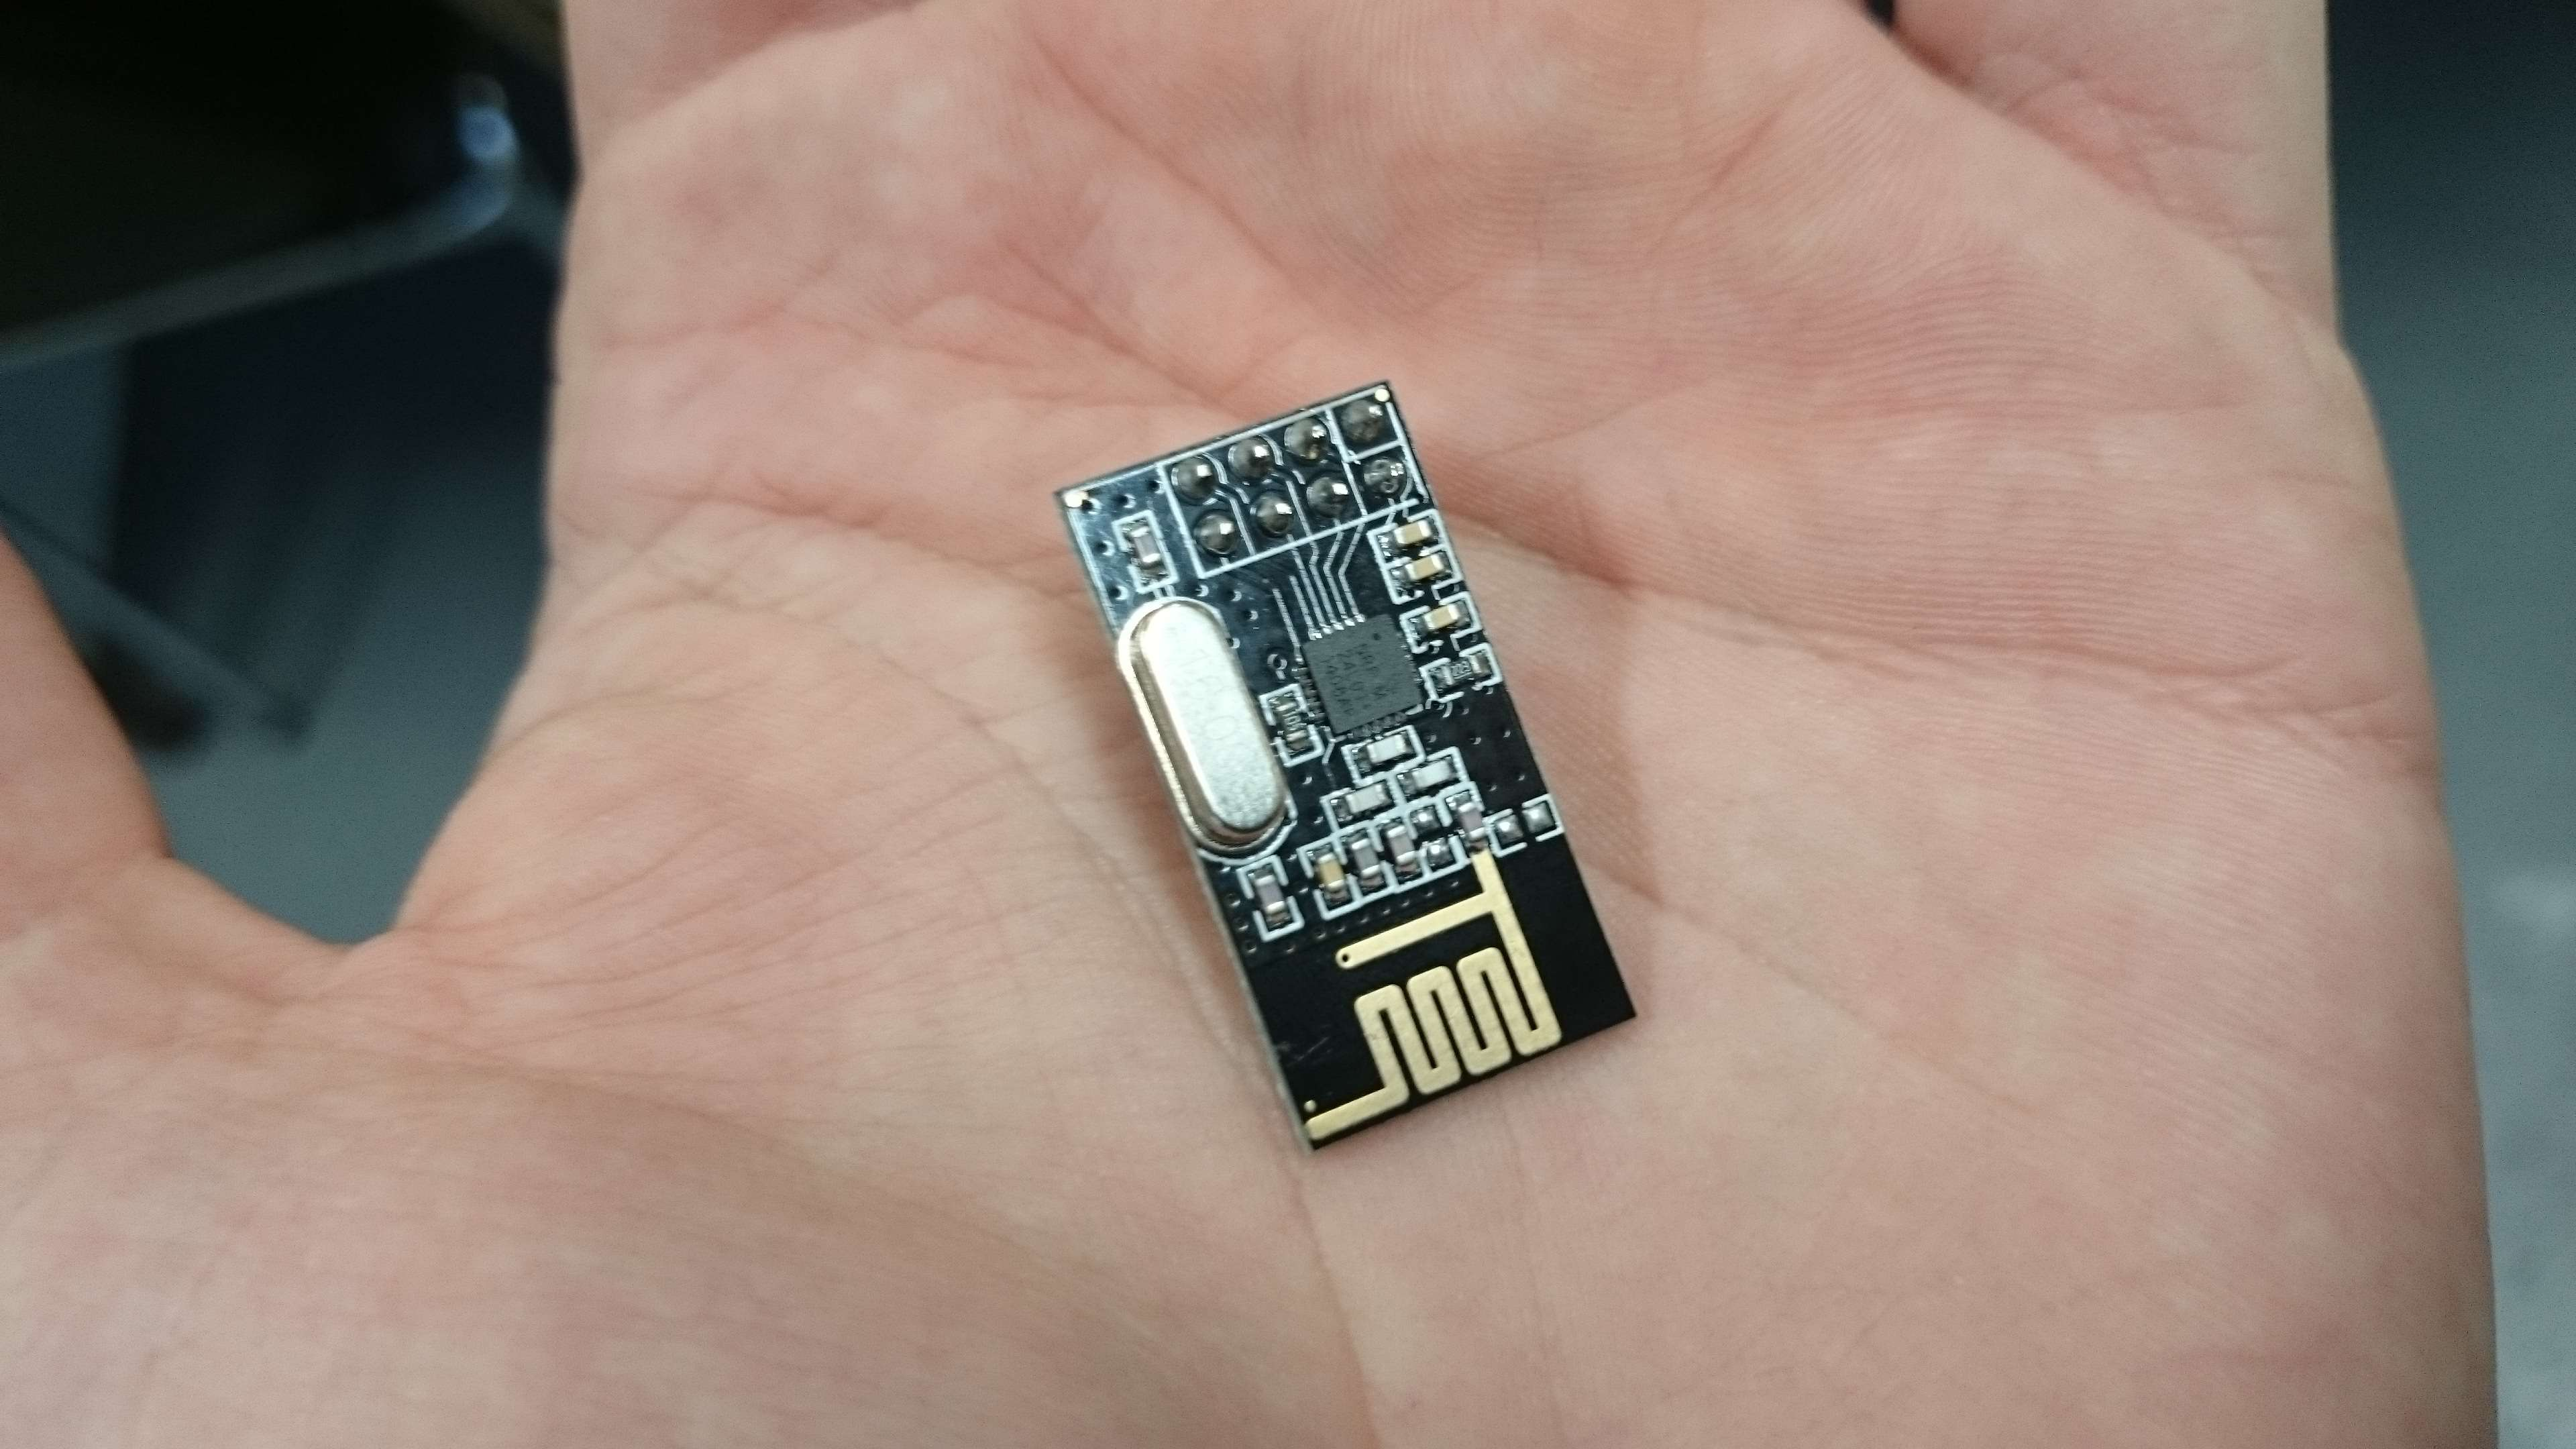
\includegraphics[scale = 0.35]{img/nrf24l01.jpg}
	  \caption{Module de communication sans fil NRF24L01}
	  \label{nrf24l01}
	\end{figure}
      
      \subsection{Contrôle moteur}
	La plupart des drones implémentent un Electronic Speed Controler (ESC) pour chaque moteur. Ces composants servent à contrôler 
	la vitesse du moteur ainsi que son sens de rotation. Il faut savoir qu'un ESC vaut environ 16 \euro. Ce qui fait 64 \euro pour 
	un quadcopter. Outre le prix important de ces modules, leur poids (25 grammes/module) aussi nous oblige à nous orienter vers 
	une autre solution. Nous avons donc pensé à créer notre propre ESC à l’aide d’un \textit{MOFSET}, de composants basiques 
	(condensateurs, résistances,...) et l’\textit{Arduino}.
	
    \section{Circuit}
      Pour pouvoir assembler tous ces composants il faut réaliser le circuit imprimé. Pour cela nous avons utilisé le logiciel Fritzing.
      C'est un logiciel libre qui permet de réaliser des schémas électroniques ainsi que le PCB associé. Ce logiciel propose un large
      catalogue de base mais il est aussi possible de créer ses propres composants. Aussi, un grand nombre de personnes utilisent ce
      logiciel, ce qui permet dans la plupart des cas de ne pas avoir à créer de composants puisqu'il y a de grandes chances que des
      utilisateurs les aient déjà dessinés.
      
      La figure \ref{schema1drone} représente le schéma électronique de notre drone et la figure \ref{pcb1drone} le PCB associé.
      
      \begin{figure}[htbp]%Schéma du premier drone
	\centering
	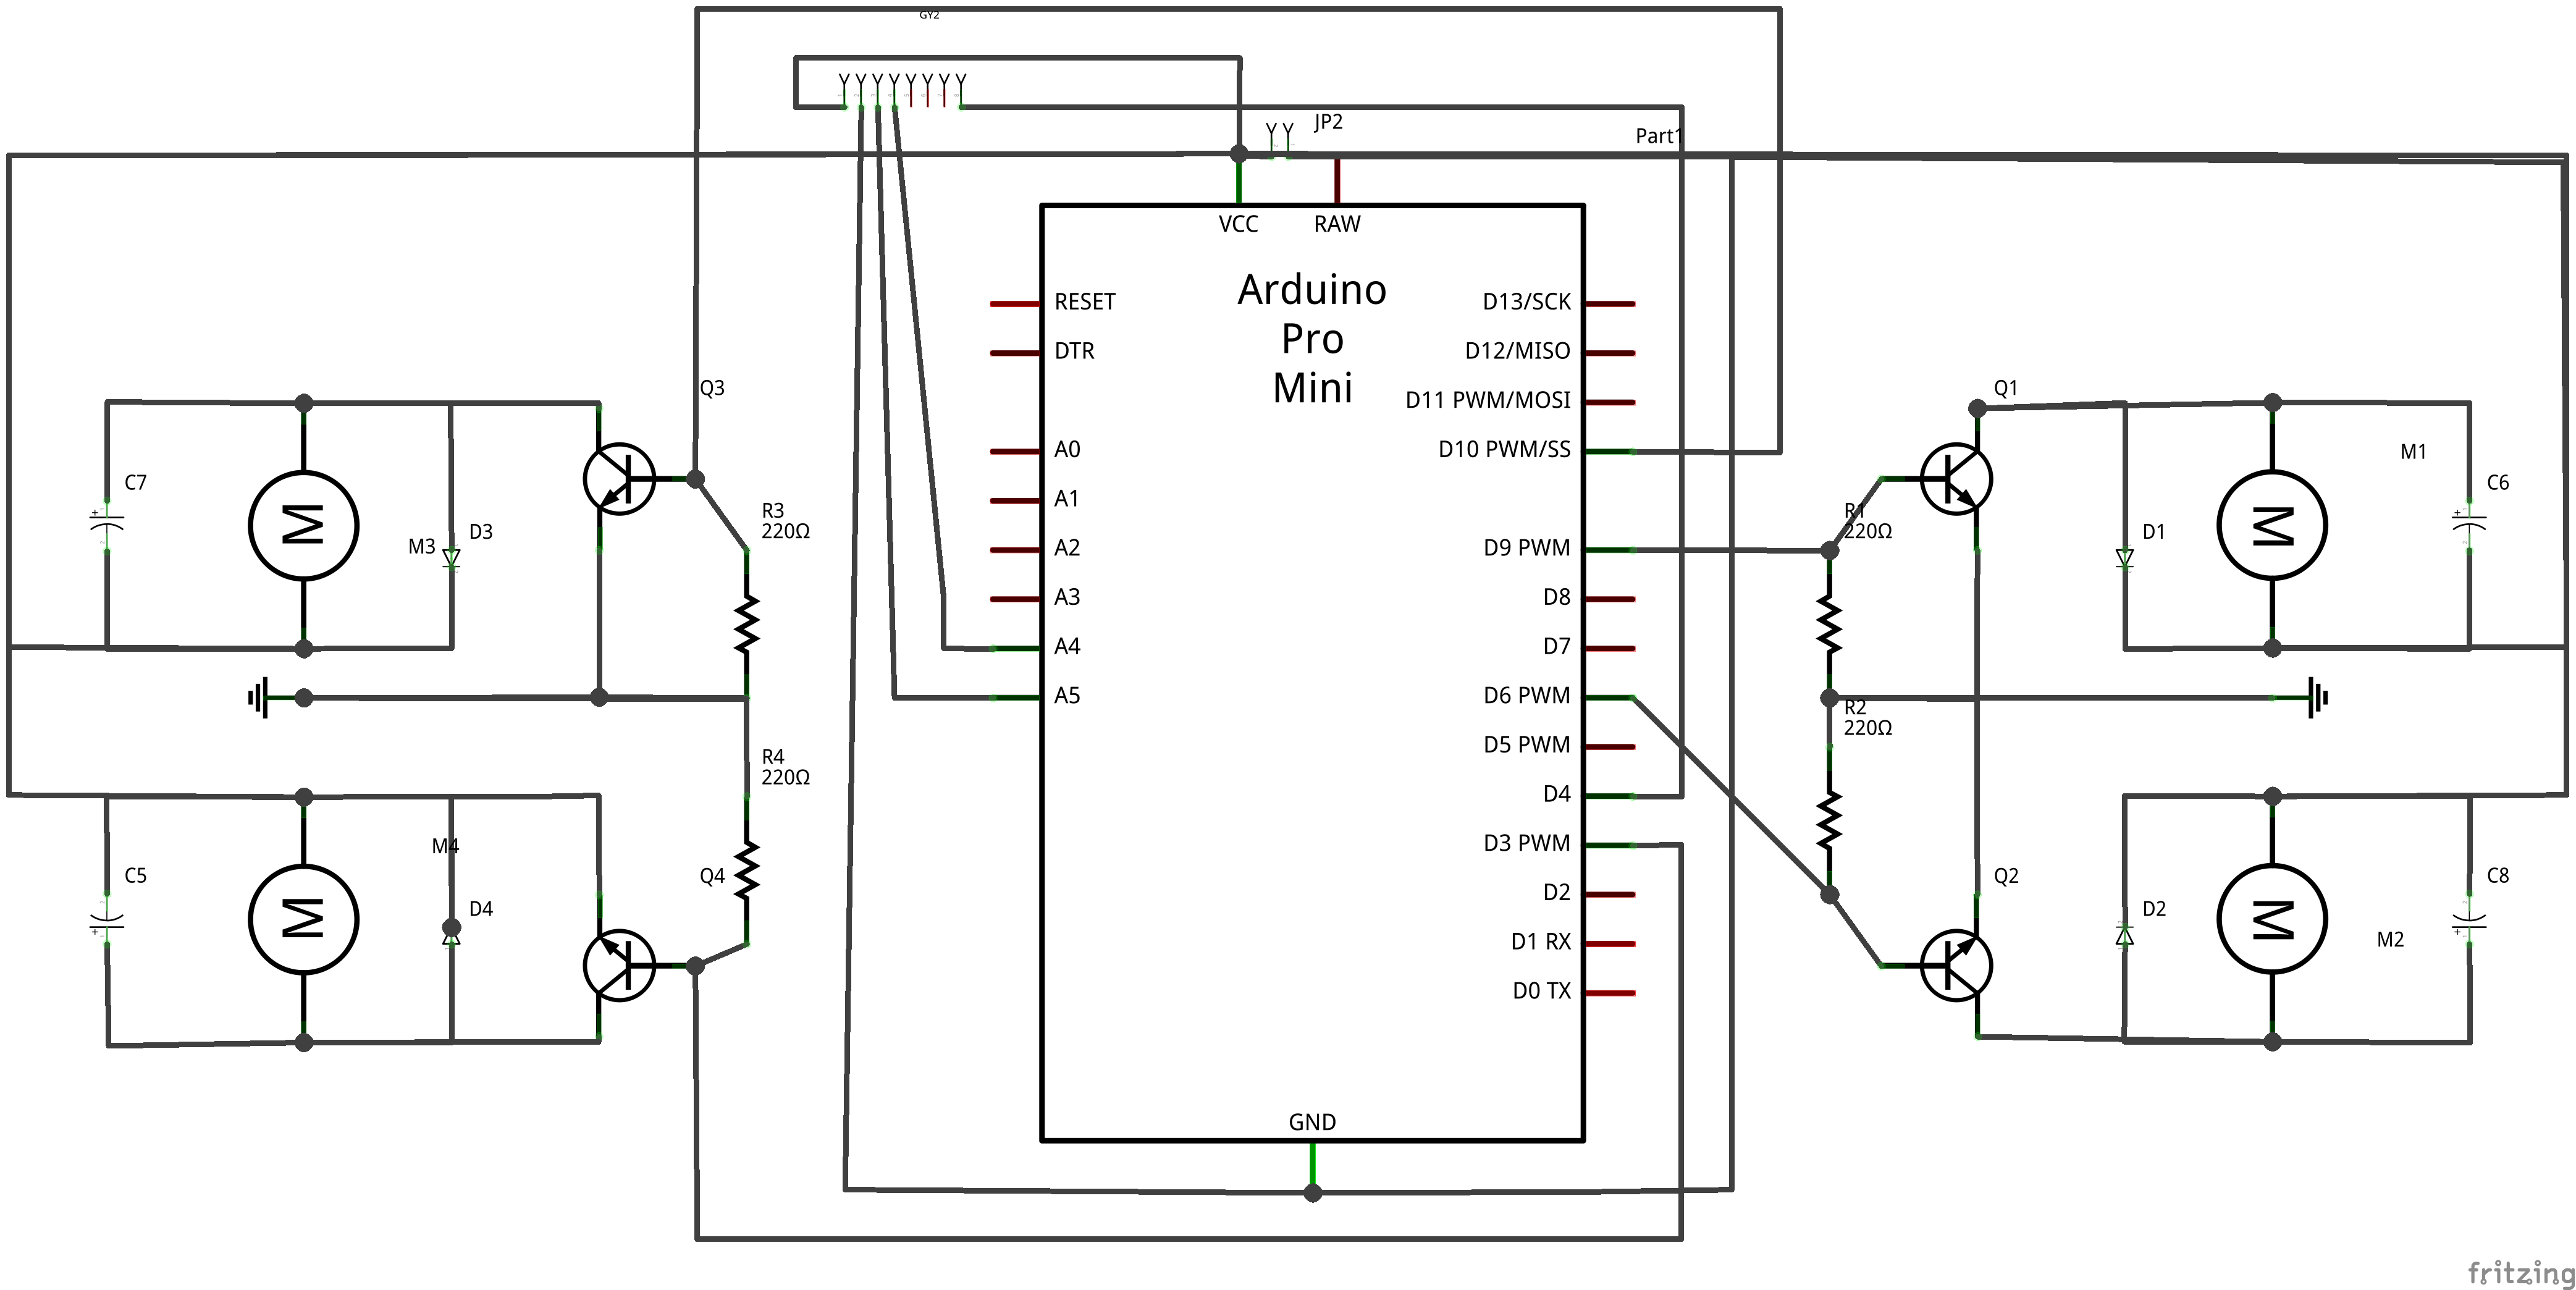
\includegraphics[scale = 0.3]{img/drone1_circuit_schema.png}
	\caption{Schéma du premier drone}
	\label{schema1drone}
      \end{figure}
      
      \begin{figure}[htbp]%PCB du premier drone
	\centering
	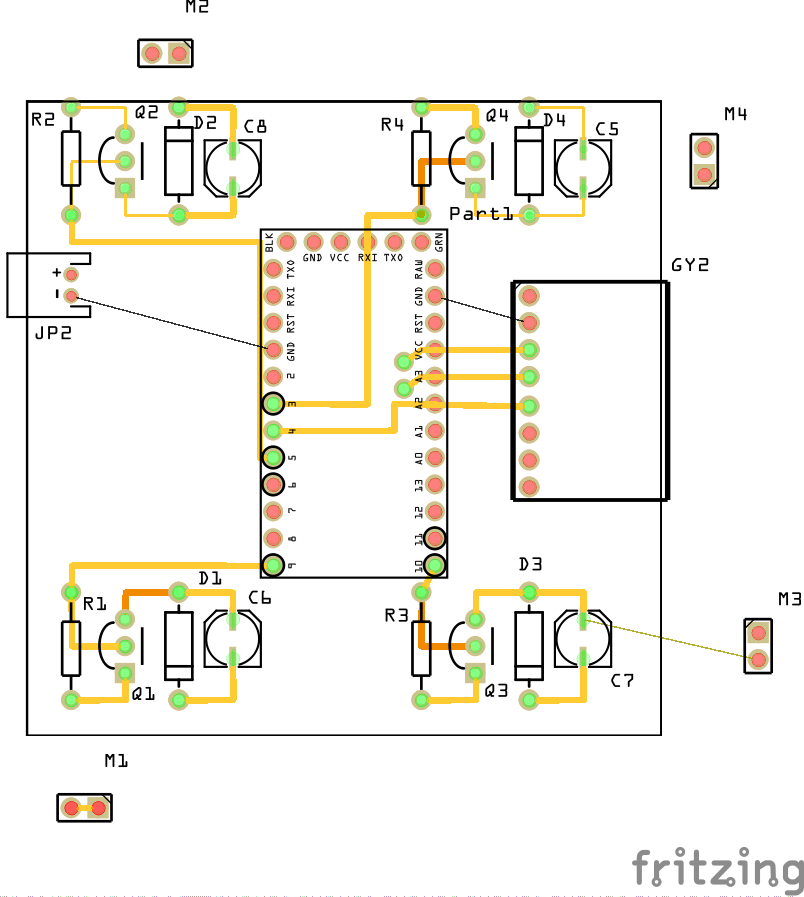
\includegraphics[scale = 0.8]{img/drone1_circuit_pcb.png}
	\caption{PCB du premier drone}
	\label{pcb1drone}
      \end{figure}
      
      \newpage
      Nous avons fait le choix de ne pas utiliser de châssis. Ces composants sont assez compliqués à choisir, car il faut choisir entre
      un matériau léger mais coûteux et un matériau "lourd" et bon marché. Donc nous avons pensé que le circuit pourrait lui-même faire
      office de châssis. Bien entendu, ce choix est risqué car le drone est plus fragile. Mais notre application n'est pas vraiment
      "à risque" dans le sens où notre drone n'est pas censé faire des acrobaties et que nous comptions mettre en place des sécurités
      pour qu'il évite les obstacles de son environnement.
      
      Avec les technologies choisis, on s'en sort pour environ 23 \euro de composants pour un drone. Le kit complet du crazyflie coûte
      à peu près 120 \euro. Nous comptions sur le fait que notre drone soit plus lourd (environ 35 grammes) que le \textit{Crazyflie} 
      (19 grammes) pour se ramener à un vol un peu moins agressif, mais cela n'a pas fonctionné. Aussi la batterie utilisée n'est pas
      intéressante en terme d'autonomie et fournit une tension de 3.3 Volts. Cependant les capteurs ultrason que nous comptions utiliser
      fonctionnent en 5 volts. Il nous a donc fallu changer aussi de batterie, ce qui nous a obligé à revoir beaucoup de choses. Car le type
      de batterie qu'il nous faut est plus lourd, ce qui implique de changer les moteurs. Ceci nous entraîne à la création d'un deuxième
      drone.
      
  \chapter{Deuxième drone}

  \listoffigures
  
  \raggedright
  \bibliographystyle{unsrt}
  \bibliography{biblio}
\end{document}          
